\documentclass[10pt]{article}
\usepackage{icmlko}

\icmlmeta{IP 파운데이션 월드모델}{137}{판의 사분의 일은 집단 순서였다}{노트 136이 팝업에서 찾은 인공물을 전 도메인에 걸어 봤다 --- 순위 기준 자체가 걸렸다}

\begin{document}

\twocolumn[
\icmlheader

\begin{abstract}
노트 136이 팝업에서 ``합친 순위 상관이 집단 간 순서를 잰다''를 찾고 가드로
만들었다. 그 가드를 \textbf{나머지 여덟 도메인에 걸어 봤다.} 도메인마다
라벨 눈금이 기계적으로 갈릴 만한 표지를 후보로 세우고(연재 종료 여부 · 무료
유료 · 매체 · 포맷 · 국가 · 플랫폼 수) 집단 안 순위로 다시 쟀다.
\textbf{둘이 걸렸다.} 웹툰을 연재 종료 여부로 가르면 $+$0.253이
$+$0.081로, 모바일을 무료/유료로 가르면 $+$0.427이 $+$0.237로 떨어진다.
차가 각각 $+$0.171과 $+$0.191이다. 그리고 그 둘이 후행 표본 711과 441로
\textbf{판 가중의 44\%}다. 판 $\rho$를 집단 보정으로 다시 계산했다 ---
챔피언이 $+$0.4328에서 \textbf{$+$0.3552}로, 축을 안 붙인 기본이 $+$0.3363에서
$+$0.2335로 내린다. \textbf{판 $\rho$의 사분의 일이 ``이게 연재 중인가''
``이게 무료 앱인가''를 맞힌 몫이었다.} 다만 두 가지가 다행이다. 첫째,
\textbf{순위는 살아남는다} --- 여섯 설정의 서열이 마지막 두 칸(차이 0.0001)만
빼고 그대로다. 이 판에서 내린 채택 결정은 전부 유효하다. 둘째, 보정하면
\textbf{축의 값어치가 오히려 커진다} --- 기본에서 검색$+$달력까지의 이득이
$+$0.0965에서 \textbf{$+$0.1217}이 된다. 인공물이 축으로는 못 올리는
바닥이라서 그것을 빼면 축이 한 일이 더 또렷해진다.
\end{abstract}
]

\begin{figure*}[t]
\centering
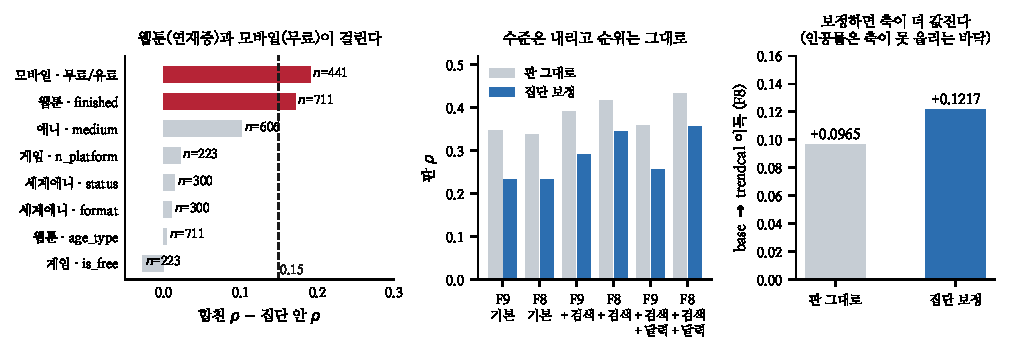
\includegraphics[width=\textwidth]{figs/corr.pdf}
\caption{왼쪽 --- 도메인마다 표지를 물려 본 것. 가운데 --- 판을 보정하면
수준은 내리고 순위는 그대로. 오른쪽 --- 보정하면 축의 이득이 커진다.}
\end{figure*}

\section{가드를 나머지 도메인에 걸었다}

노트 136의 가드는 팝업에서 만들었고 팝업에서만 검정했다. 판 $\rho$가 아홉
도메인의 가중평균이니, 같은 인공물이 다른 도메인에도 있으면 \emph{순위
기준 자체}가 걸린다.

도메인마다 ``라벨 눈금이 기계적으로 갈릴 만한'' 표지를 후보로 세웠다.

\begin{table}[t]
\centering\tsize
\caption{F9 짝 순위 · 검색$+$달력. 차 $=$ 합친 $\rho$ $-$ 집단 안 $\rho$.}
\begin{tabular}{llrr}
\toprule
& 표지 & $n$ & 차 \\
\midrule
\textbf{모바일} & 무료/유료 & 441 & \textbf{$+$.191} \\
\textbf{웹툰} & 연재 종료 & 711 & \textbf{$+$.171} \\
애니 & 매체 & 606 & $+$.102 \\
게임 & 플랫폼 수 & 223 & $+$.022 \\
세계애니 & 상태 & 300 & $+$.015 \\
세계애니 & 포맷 & 300 & $+$.010 \\
웹툰 & 연령등급 & 711 & $+$.004 \\
게임 & 무료 여부 & 223 & $-$.027 \\
\bottomrule
\end{tabular}
\end{table}

\claimx{\textbf{둘이 걸렸고 하필 큰 둘이다.} 웹툰(711)과 모바일(441)이
후행 2{,}614건 중 1{,}152건, \textbf{판 가중의 44\%}다.}{둘 다 기제가
뻔하다 --- 연재 중인 웹툰은 즐겨찾기가 덜 쌓였고, 무료 앱은 유료 앱보다
평점 수가 훨씬 많다. 모형이 축과 달력으로 그 구분을 맞히고 있고, 그것이
합친 순위에 들어간다.}

게임의 무료 여부가 $-$0.027로 음수인 것도 말이 된다 --- 스팀에서 무료
게임의 리뷰 수는 유료와 크게 안 갈린다.

\section{그래서 판을 다시 계산했다}

\begin{table}[t]
\centering\tsize
\caption{판 $\rho$. 보정은 걸린 도메인만 집단 안 순위로 다시 잰 것.}
\begin{tabular}{lrrr}
\toprule
& 그대로 & 집단 보정 & 차 \\
\midrule
F9 기본 & $+$.3464 & $+$.2328 & $-$.114 \\
F8 기본 & $+$.3363 & $+$.2335 & $-$.103 \\
F9 $+$검색 & $+$.3902 & $+$.2906 & $-$.100 \\
F8 $+$검색 & $+$.4170 & $+$.3442 & $-$.073 \\
F9 $+$검색$+$달력 & $+$.3576 & $+$.2549 & $-$.103 \\
\textbf{F8 $+$검색$+$달력} & \textbf{$+$.4328} & \textbf{$+$.3552} & $-$.078 \\
\bottomrule
\end{tabular}
\end{table}

\claimx{\textbf{판 $\rho$의 사분의 일이 집단 순서였다.} 챔피언이 $+$0.4328에서
$+$0.3552로, 기본이 $+$0.3363에서 $+$0.2335로 내린다. 노트 125부터 지금까지
보고한 판 수치는 전부 이만큼 높았다.}{``보정한 값이 참값''이라는 뜻은
아니다. 집단 안 순위로 바꾸는 것은 집단 간 정보를 \emph{전부} 버리는
극단이고, 그중 일부는 진짜 예측일 수 있다. 참값은 두 값 사이 어딘가다.}

\section{다행인 것 둘}

\claimx{\textbf{순위가 살아남는다.} 보정 전후로 여섯 설정의 서열이 마지막
두 칸만 바뀐다 --- 그 둘은 F9 기본($+$0.2328)과 F8 기본($+$0.2335)으로
차이가 0.0001이다. \textbf{이 판에서 내린 채택 결정은 전부 유효하다.}}{여섯
설정에서만 확인했다. 보정이 순위를 바꾸는 설정이 어딘가 있을 수 있다 ---
그래서 앞으로는 실행마다 보정값을 같이 기록한다.}

\claimx{\textbf{보정하면 축이 더 값진다.} 기본에서 검색$+$달력까지의 이득이
$+$0.0965에서 \textbf{$+$0.1217}이 된다. 인공물은 축으로 올릴 수 없는
바닥이라, 그것을 빼면 축이 한 일의 비중이 커진다.}{같은 논리로, 앞으로
축을 더 붙여 얻을 수 있는 여지도 보정된 눈금에서 봐야 한다. 보정 판이
$+$0.3552이니 위쪽 여유가 그대로 남아 있다.}

\section{규약}

실행마다 \texttt{board\_grp}(집단 보정 판 $\rho$)를 요약에 남기도록 했다.
순위 기준은 그대로 둔다 --- 지금까지의 이력이 전부 그 눈금 위에 있고,
순위가 보정에 안 흔들리는 것을 확인했기 때문이다. \textbf{다만 수준을
말할 때는 보정값을 쓴다.}

\begin{table}[t]
\centering\tsize
\caption{남은 것.}
\begin{tabular}{ll}
\toprule
표지 & 후보를 손으로 세웠다 --- 놓친 것이 있을 수 있다 \\
중간값 & 집단 안 순위는 극단이다. 부분 보정이 필요 \\
애니 & 차 $+$.102 로 문턱 아래지만 작지 않다 \\
\bottomrule
\end{tabular}
\end{table}

둘째 줄이 제일 걸린다. 지금 보정은 집단 간 정보를 전부 버리는데, 어떤
작품이 극장판인지 TV인지는 \emph{기획 단계에 아는 것}이라 예측에 써도
되는 정보다. 무료 앱인지도 마찬가지다. \textbf{버려야 할 것은 ``집단을
맞혔다''는 공짜 점수이고, 남겨야 할 것은 ``집단 안에서 순서를 맞혔다''인데,
지금 방식은 둘을 같이 버린다.} 다음은 그 중간을 만드는 일이다.

\end{document}
